%%%%%%%%%%%%%%%%%%%%%%%%%%%%%%%%%%%%%%%%%
% Structured General Purpose Assignment
% LaTeX Template
%
% This template has been downloaded from:
% http://www.latextemplates.com
%
% Original author:
% Ted Pavlic (http://www.tedpavlic.com)
%
% Note:
% The \lipsum[#] commands throughout this template generate dummy text
% to fill the template out. These commands should all be removed when
% writing assignment content.
%
%%%%%%%%%%%%%%%%%%%%%%%%%%%%%%%%%%%%%%%%%

%----------------------------------------------------------------------------------------
%	PACKAGES AND OTHER DOCUMENT CONFIGURATIONS
%----------------------------------------------------------------------------------------

\documentclass{article}

\usepackage{fancyhdr} % Required for custom headers
\usepackage{lastpage} % Required to determine the last page for the footer
\usepackage{extramarks} % Required for headers and footers
\usepackage{graphicx} % Required to insert images
\usepackage{lipsum} % Used for inserting dummy 'Lorem ipsum' text into the template
\usepackage{natbib} % bibliography
\usepackage{filecontents}
\usepackage{pgfplots}
\usepackage{pgfplotstable}
\usepackage{siunitx}
\pgfplotsset{compat=1.5}

% Margins
\topmargin=-0.45in
\evensidemargin=0in
\oddsidemargin=0in
\textwidth=6.5in
\textheight=9.0in
\headsep=0.25in

\linespread{1.1} % Line spacing

% Set up the header and footer
\pagestyle{fancy}
\lhead{\hmwkClass:\ \hmwkTitle} % Top left header
\chead{} % Top center header
\rhead{\firstxmark} % Top right header
\lfoot{\lastxmark} % Bottom left footer
\cfoot{} % Bottom center footer
\rfoot{Page\ \thepage\ of\ \pageref{LastPage}} % Bottom right footer
\renewcommand\headrulewidth{0.4pt} % Size of the header rule
\renewcommand\footrulewidth{0.4pt} % Size of the footer rule

\setlength\parindent{0pt} % Removes all indentation from paragraphs

%----------------------------------------------------------------------------------------
%	DOCUMENT STRUCTURE COMMANDS
%	Skip this unless you know what you're doing
%----------------------------------------------------------------------------------------

% Header and footer for when a page split occurs within a problem environment
\newcommand{\enterSectionHeader}[1]{
\nobreak\extramarks{#1}{#1 continued on next page\ldots}\nobreak
\nobreak\extramarks{#1 (continued)}{#1 continued on next page\ldots}\nobreak
}

% Header and footer for when a page split occurs between problem environments
\newcommand{\exitSectionHeader}[1]{
\nobreak\extramarks{#1 (continued)}{#1 continued on next page\ldots}\nobreak
\nobreak\extramarks{#1}{}\nobreak
}

\newcommand{\mainSectionName}{}
\newenvironment{mainSection}[1]{ % Makes a new environment called homeworkProblem which takes 1 argument (custom name) but the default is "Problem #"
\renewcommand{\mainSectionName}{#1} % Assign \homeworkProblemName the name of the problem
\section{\mainSectionName} % Make a section in the document with the custom problem count
\enterSectionHeader{\mainSectionName} % Header and footer within the environment
}{
\exitSectionHeader{\mainSectionName} % Header and footer after the environment
}

%----------------------------------------------------------------------------------------
%	NAME AND CLASS SECTION
%----------------------------------------------------------------------------------------

\newcommand{\hmwkTitle}{Market Chirp} % Assignment title
% \newcommand{\hmwkDueDate}{Monday,\ January\ 1,\ 2012} % Due date
\newcommand{\hmwkClass}{ABCs} % Course/class
\newcommand{\hmwkAuthorName}{Alex Fong, Brandon Woo, Chris Konstad, Sakib Shaikh} % Your name

%----------------------------------------------------------------------------------------
%	TITLE PAGE
%----------------------------------------------------------------------------------------

\title{
\vspace{2in}
\textmd{\textbf{\hmwkClass:\ \hmwkTitle}}\\
\vspace{3in}
}

\author{\textbf{\hmwkAuthorName}}
\date{December 3rd, 2015} % Insert date here if you want it to appear below your name

%----------------------------------------------------------------------------------------
% Bibliography
\begin{filecontents*}{ABCs.bib}
@MISC{GitBranching,
  author = {{Keith D. Gregory}},
  title = {{Practical Git: A Workflow to Preserve Your Sanity}},
  note = {[Online; accessed Nov 30, 2015]},
  url = {http://www.kdgregory.com/images/scm.git/02-fishbone.gif}
}
\end{filecontents*}
%------------------------------------------------------------------------------

%------------------------------------------------------------------------------
% USER ARRIVAL RATES
\begin{filecontents}{users.temp}
X,Y
0,1
30,2
60,4
90,8
120,16
150,32
180,64
210,128
240,256
270,512
\end{filecontents}
%------------------------------------------------------------------------------

\begin{document}

\maketitle

%----------------------------------------------------------------------------------------
%	TABLE OF CONTENTS
%----------------------------------------------------------------------------------------

%\setcounter{tocdepth}{1} % Uncomment this line if you don't want subsections listed in the ToC

\newpage
\tableofcontents
\newpage

%----------------------------------------------------------------------------------------
%	PROBLEM 1
%----------------------------------------------------------------------------------------

% To have just one problem per page, simply put a \clearpage after each problem

%\begin{homeworkProblem}
\begin{mainSection}{Introduction}
Market Chirp is a stock recommendation web application developed in the context of UCLA CS 188/219, Scalable Internet Services in Fall 2015 by the team ABCs. The application analyzes Twitter's sentiment on all NASDAQ stocks and provides the user with the information required to make sound investment decisions.
\\
\subsection{What we do} % TODO This should just be a statement, not an explanation
\indent Market Chirp analyzes over 2,800 stocks in the New York Stock Exchange. Once a user creates an account, an aggregate of data appears in the dashboard. In the dashboard after selecting a stock, one can view the Twitter feed, the tweet sentiment of the stock, and the stock history. Common stock data such as the market cap and current versus historical stock price is gathered from Yahoo! Finance's API. In addition, Market Chirp takes a mix of the most influential and most recent tweets containing the current stock ticker's symbol of the past twenty-four hours and runs the tweets through a sentiment analyzer. The average of the sentiments is displayed along with a tweet that most closely matches the sentiment.
\\
\indent In addition, one can favorite stocks to keep a running list of stocks to view with ease at later times. The favorited stocks appear in the sidebar and can be unfavorited at anytime.
\\
\subsection{Our goal}
\indent The goal of Market Chirp is to quickly analyze the public's opinion of high-quality stocks through short notes on Twitter. Since the feed of Tweets is queried in real time when a user searches for a certain stock, the sentiment analysis of a stock is the public's current opinion of is a stock is bullish or bearish. For example, if a stock is on the downhill trend for its market price but its Twitter sentiment is on the uptrend, one may take that as an indication to buy the stock since more people will then value the stock higher. Market Chirp's ultimate goal is not to predict the stock market as the sentiment is based only on the dataset of people tweeting about a stock but is to give insight on the predicted future of stocks based on public opinion.
\\
\subsection{How we do it}
\indent Market Chirp is implemented in Ruby on Rails (Ruby 2.2.1 and Rails 4.2.4). The backend data store is a relational database management system, in our case MySQL. Since the purpose of CS 188/219: Scalable Internet Services is to build and deploy a scalable web service, this report will therefore discuss the deployment, performance and scalability of Market Chirp.
\end{mainSection}

\begin{mainSection}{Development Process}
\begin{figure}[htpb]
  \centering
  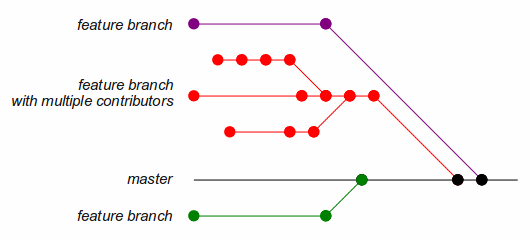
\includegraphics[width=0.75\columnwidth]{resources/git.jpg} % Example image
  \caption{Example of our Git branching technique (\cite{GitBranching})}
  \label{fig:git}
\end{figure}
\subsection{Planning}
Through the development of Market Chirp, our team used an Agile framework. Here we had weekly sprint planning meetings to discuss where the project was headed along with retrospective meetings to gain a perspective of what we had accomplished or still had yet to implement over the past week. Tasks not completed by the specified sprint date were automatically moved into a backlog or icebox in order to be completed in future sprints. By using these stand-up meetings, our team was able to precisely figure out the tasks that needed to be finished and how our individual features were pushed into the big picture of the entire product and its scalability.
\\

\subsection{Scheduling}
Pivotal Tracker guided us in following the Agile development framework. With Pivotal Tracker integrated with Github to keep track of certain features or issues, our commits and releases could be synced up to reflect the current status of the application. We were able to assign tickets to certain people in order to split the work up in an efficient manner. By modularizing the tasks, implementing the features and bug fixes was more smooth that using another development framework such as Waterfall Planning. As the quarter moved along however, Pivotal Tracker started being faded out as we were in constant connection with each other still keeping up to date where we should be with the project.
\\

\subsection{Automated testing}
Since Rails is a test driven development framework, it automatically created testing templates for the classes we developed. We made sure to follow test driven development in which one creates test cases for a feature before actually implementing the feature. By following TDD, edge cases were covered as we programmed out the features since we were aware of them beforehand. Since we created ample test cases, the majority of our code was covered and allowed us to be confident our website would not crash when scaled upward.
\\

Travis CI was set up as a continuous integration service for building and testing project. We created numerous test cases that would be run each commit to see the version control's reliability. Connecting Travis CI to Github allowed us to keep commiting new code and test its reliability and keep it bug free.
\\
\subsection{Version control}
Our version control management system was Git. By keeping the master branch as our production branch, our releases on AWS were always in sync with the latest release on our remote Github. We all worked on separate branches and used pull requests to merge our new code into the other branches eventually merging into master. By constantly rebasing our branches, our development history is clean and looks as though only one person had developed it. Separating the features and bug fixes into their own respective branch allowed each developer to focus on his own feature without conflicting with other developers. After merging in the features, the application's version control was clean.
\\

\subsection{Pair programming}
We also performed pair programming in certain scenarios such as when developing our Memcached feature optimization. Pair programming allowed us to minimize our errors as we wrote our code since we had multiple eyes on the screen at a time. In doing so, our time of outlining a feature branch to pushing production ready code was optimized a substantial amount.
\\
\end{mainSection}

\begin{mainSection}{Testing}
  \subsection{Server configuration}
  We used the following software packages for all of our testing:
  \begin{itemize}
    \item Nginx
    \item Phusion Passenger
    \item MySQL
  \end{itemize}

  We modified the provided JavaScript Object Notation (JSON) files to configure our server with the proper environmental variables, letting us keep our secret keys out of our public version control.\\

  The service was developed on our personal laptops, with all performance testing running on Amazon Web Services (AWS).  It was trivial for us to deploy new versions because we only had to deploy for performance testing, which was handled by our server provisioning scripts.\\

\begin{figure}[htpb]
  \begin{center}
    \begin{tabular}{| l | r | r | r | }
      \hline
      \multicolumn{4}{ |c| }{M3 Server Configurations}\\
      \hline
      Server Size & Cores & RAM (GiB) & Process Parallelization\\
      \hline
      Med     & 1 &  3.75 & 1 \\
      Large   & 2 &  7.50 & 2 \\
      XLarge  & 4 & 15.00 & 4 \\
      2XLarge & 8 & 30.00 & 8 \\
      \hline
    \end{tabular}
    \caption{Table of server configurations.  These settings were used for all tests.  For a server with $n$ cores, $n$ worker processes were used.  Each worker process was single threaded.}
    \label{tab:m3}
  \end{center}
\end{figure}

Figure \ref{tab:m3} shows the configurations of the various server sizes used for all testing.  By minimizing differences in the testing setups, we were able to clearly show the effects of each optimization.\\

When separate database servers were used (for example, in horizontal scaling), the database server was the same size as the application server (\texttt{db.m3med} was used for \texttt{m3.med}).

  \subsection{User simulation}
  \begin{figure}[htpb]
    \begin{center}
      \begin{tikzpicture}
        \begin{axis}[title=Test User Arrival Rates,
            xlabel = Time (sec),
            ylabel = Users/sec,
            legend pos = outer north east,
          ]
          \addplot[thick, orange] table [
              col sep=comma,
              x = X,
              y = Y,
            ] {users.temp};
        \end{axis}
      \end{tikzpicture}
    \end{center}
    \caption{Graph showing the number of test users sent from our Tsung server to our application server throughout the duration of the performance tests.}
    \label{graph:users}
  \end{figure}

  Our Tsung tests used the test user arrival rates shown in Figure \ref{graph:users}.\\

  Missing our slowest level of caching, our MySQL "caches" of Twitter sentiment data, and to a lessen extent Yahoo Finance data, causes $20+$ second delays.  Because of these unreasonably long delays, our service would have worker processes keeping those caches warm if we deployed this to the real world.  To simulate this effect in our tests, we limited our test users to interacting with a small subset of the real world stocks.  According to our tests, useres only care about Apple, Facebook, Google and Tesla stocks, which is unrealistic.  Another benefit of focusing on popular stocks is that we are guaranteed to always have enough Twitter data about each stock symbol.  Some of the less popular stock symbols would have 5 tweets or less, making both the data inaccurrate and the request too easy to strain the system.\\


  \subsection{Critical Path}
  Our critical path through our application was the path that we thought the average user was most likely to hit.  We had two user models, with a 50\% chance that either model was selected for each test user:
  \begin{enumerate}
    \item A user who is not logged in
    \item A user who is logged in
  \end{enumerate}

  While visiting each page, the test user would wait a randomized amount of time up to a threshold to emulate a person either looking at the page or filling out forms.

  \subsubsection{User not logged in}
  A user who is not logged in has no account on Market Chirp and therefore has no favorites.  They are also unable to access the Dashboard feature, which is the page that requires the most data fetching and handling, making it the most expensive page to load.  Instead, this user:
  \begin{enumerate}
    \item Visits our homepage
    \item Visits our sentiment analysis page
    \item Searchs for FB
    \item Searches for AAPL
    \item Searches for GOOGL
    \item Searches for TSLA
    \item Visits our stock data page
    \item Searchs for FB
    \item Searches for AAPL
    \item Searches for GOOGL
    \item Searches for TSLA
  \end{enumerate}

  \subsubsection{User is logged in}
  A logged in user would want to check their favorited stocks, which is most easily done through the Dashboard page.  From there, we thought the average user would check their stocks, look for a new one, favorite the new stock and drop one of their favorited stocks.  This user:
  \begin{enumerate}
    \item User logs in
    \item Visits their dashboard
    \item Visits the dashboard for GOOGL
    \item Favorites GOOGL
    \item Visits the dashboard for TLSA
    \item Visits the dashboard for FB
    \item Visits the dashboard for AAPL
    \item Removes AAPL from their favorite list
    \item User logs out
  \end{enumerate}

  \subsection{Initial testing}
  The first tests of Market Chirp showed massive performance issues.  Twitter sentiment data was calculated for all 100 tweets (pulled from Twitter separately for each request), leading to $20+$ second delays in getting results when searching for a stock symbol.  From looking at the logs and \texttt{top}, it was clear that the process was CPU bound.  No formal Tsung testing happened at this performance level because individual page loadings took too long and the service was not ready for even a single user.\\

  A MySQL driven "cache" was created to store Twitter analysis data for a day, for each stock that was searched.  While initial stock searches caused unreasonable delays of $20+$ seconds, subsequent delays were much, much faster, happening in less than $5$ seconds.  The cache stores the overall calculated sentiment and it stores a single tweet out of the $100$ sampled tweets that has the closest sentiment value as an average tweet for the given sample.\\

  A similar MySQL driven caching system as added to cache the 10 years of Yahoo Finance stock data downloaded for each symbol requested.  The stock data itself was stored as a JSON text blob, as the client side graphing library read in that JSON.  It made more sense to store the JSON received from Yahoo in the same format that the graph required, than it did to parse the JSON, store each value individually, and read those values out as JSON later.

  \subsection{Vertical scaling}
  Vertical scaling, simply throwing more processing power at the problem, is simple but expensive.  We expected to get marginal performance gains by scaling vertically because our main bottleneck was the CPU bound Twitter sentiment analysis.

  \begin{center}
  \begin{tikzpicture}
    \begin{axis}[title=Vertical Scaling,
        xlabel = Time (sec),
        ylabel = 200/sec,
        legend pos = outer north east,
      ]
      \addplot[thick, orange] table [
              col sep=comma,
              x = X,
              y = Y,
            ] {resources/m3med/data/200.csv};
      \addplot[thick, blue] table [
              col sep=comma,
              x = X,
              y = Y,
            ] {resources/m3large/data/200.csv};
      \addplot[thick, green] table [
              col sep=comma,
              x = X,
              y = Y,
            ] {resources/m3xlarge/data/200.csv};
      \addplot[thick, magenta] table [
              col sep=comma,
              x = X,
              y = Y,
            ] {resources/m32xlarge/data/200.csv};
      \addlegendentry{M3 Med}
      \addlegendentry{M3 Large}
      \addlegendentry{M3 XLarge}
      \addlegendentry{M3 2XLarge}
      \end{axis}
    \end{tikzpicture}
  \end{center}

  \subsection{Horizontal scaling}
  \begin{center}
  \begin{tikzpicture}
    \begin{axis}[title=Horizontal Scaling,
        xlabel = Time (sec),
        ylabel = 200/sec,
        legend pos = outer north east,
      ]
      \addplot[thick, orange] table [
              col sep=comma,
              x = X,
              y = Y,
            ] {resources/multi_m3med/data/200.csv};
      \addplot[thick, blue] table [
              col sep=comma,
              x = X,
              y = Y,
            ] {resources/multi_m3large/data/200.csv};
      \addplot[thick, green] table [
              col sep=comma,
              x = X,
              y = Y,
            ] {resources/multi_m3xlarge/data/200.csv};
      \addplot[thick, magenta] table [
              col sep=comma,
              x = X,
              y = Y,
            ] {resources/multi_m32xlarge/data/200.csv};
      \addlegendentry{M3 Med}
      \addlegendentry{M3 Large}
      \addlegendentry{M3 XLarge}
      \addlegendentry{M3 2XLarge}
      \end{axis}
    \end{tikzpicture}
  \end{center}
\end{mainSection}

\bibliographystyle{plainnat}
\bibliography{ABCs}
\end{document}
